\begin{center}
     \Large{\textbf{AND Cheat Sheet}} \\
\end{center}

\section{Vocabulary}
\textsc{Hyperbolic eq.points} $\mathcal{R}\{x\} \neq 0$ \\
\textsc{Nonhyperbolic problems} Equilibria with EV on the imaginary axis.

\section{Basics on cont.-time dynamical systems}
\begin{align*}
\dot{x} = f(t,x,p), \quad x(t_0) = x_0 \Leftrightarrow \dx = f(x,p), \quad x(0)=x_0
\end{align*}
\subsection{Flow of a system}
Solution is the flow $\phi_t(x_0)$
\begin{align*}
x(t;x_0,p)=\phi_t(x_0,p)
\end{align*}
\textsc{Flow axioms}\\
\begin{align*}
\phi_0(x_0,p)&=x_0\\
\phi_{t_1}[\phi_{t_2}(x_0,p),p] &= \phi_{t_1+t_2}(x_0,p)
\end{align*}
\subsection{Existence and uniqueness}
\textsc{Existence and uniqueness of local (in time) solutions}\\
\emph{If $f(x)$ is smooth enough, then solutions exist and are unique. No guarantee that they exist forever - only guarantees to exist in a very short time interval around $t_0$.}\\
If $f$ is Lipschitz in $x$ and piecewise continuous in $t$ then the IVP has a unique solution $x(t)=\phi(t;t_0)x_0$ over a finite time interval $t\in[t_0-\tau,t_0+\tau]$.\\
Allows for finite-escape times/blow-up (reach infinity in finite time).

\subsection{Stability}
Def.: An equilibrium point is a state $x^*$ s.t. $f(x^*)=0$\\
Def.: An eq.point $x^*$ is stable if for any $\epsilon>0$ there exists a constant $\delta > 0$ such that \begin{align*}
\forall x_0: \Vert x_0 - x^* \Vert \leq \delta \Rightarrow \Vert x(t)-x^* \Vert \leq \epsilon \quad \forall t \geq 0
\end{align*}

\textsc{Attractor}\\
$x^*$ is attractive if $\lim_{t\rightarrow \infty} \Vert x(t)-x^* \Vert = 0 \quad \forall x_0 \in \mathcal{S}$ with $\mathcal{S}$ being the domain of attraction.\\
Eq points may be attractive without being stable (ex. Vinograd's system).

\textsc{Asymptotic stability}\\
An eq.point $x^*$ is asymptotically stable if it is stable and attractive.

\textsc{Exponential stability}\\
An eq.point $x^*$ is exponentially stable in $\mathcal{S}$ if it is stable and there are constants $a, \lambda > 0$ such that $\forall x_0 \in \mathcal{S}: \Vert x(t)-x^*\Vert \leq a\Vert x_0 - x^* \Vert e^{-\lambda t}$

\section{Linear systems}
\subsection{LTI systems}
\subsection{LTV systems and Floquet theory}
\section{Nonlinear flows}
\subsection{Local Theory}
\textsc{Hartman-Grobman}\\
The behavior of a nonlinear systems in a vicinity of hyperbolic eq. points is the same as in the linearized system around that point.

\textsc{Center manifold theorem}\\
\begin{align*}
\frac{dh}{dx_z}[A_zx_z+f_z(x_z, h(x_z))] = A_sh(x_z)+f_s(h(x_z),x_z) \\
h(0)=0, \quad \frac{dh(0)}{dx_z} = 0
\end{align*}


\subsection{Non-local phenomena}
\section{Bifurcations of vector fields}
\subsection{Bifurcations of SSs}
\textsc{Transcritical bifurcation}\\
\emph{Standard mechanism for change of stability for a fixed point which exists for all values of the parameter}.\\
Ex.: $\dot{x}=rx-x^2$.\\
Fixed point at $x^*=0 \quad \forall r$. For $r<0$ unstable fixed point at $x^*=r$ and a stable at $x^*=0$. For $r=0^-$ the fixed points unify. For $r>0$ the origin is unstable and $x^*=r$ becomes stable - \textbf{exchange of stabilities}
\begin{center}
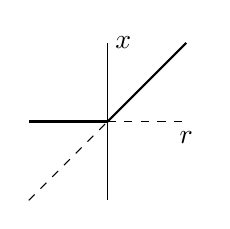
\begin{tikzpicture}
\draw (0,1.5) -- (0,-0.5);
\draw [thick](-1,0.5) -- (0,0.5);
\draw [dashed](0,0.5) -- (1,0.5);
\draw [thick](0,0.5) -- (1,1.5);
\draw [dashed](-1,-0.5) -- (0,0.5);
\node at (1,0.3) {$r$};
\node at (0.2,1.5) {$x$};
\end{tikzpicture}
\end{center}
\vspace{0.2cm}


\textsc{Saddle node bifurcation}\\
\emph{Fixed points are created and destroyed. As a parameter is varied, two fixed points move toward each other, collide and mutually annihilate}.\\
Ex: $\dot{x}=r+x^2$.\\ $r<0$: 2 FP (1 stable, 1 unstable),\\ $r=0^-$: half-stable FP, \\ $r>0$: no FP.\\ In this example the bifurcation occurred at $r=0$.
\begin{center}
\begin{tikzpicture}
\draw (0,1.5) -- (0,-0.5);
\draw (-1,0.5) -- (1,0.5);
\draw [thick](-1,-0.25) .. controls (-0.5,-0.1) and (0,0) .. (0,0.5);
\draw [dashed](-1,1.25) .. controls (-0.5,1.1) and (0,1) .. (0,0.5);
\node at (1,0.3) {$r$};
\node at (0.2,1.5) {$x$};
\end{tikzpicture}
\end{center}
\vspace{0.2cm}

\subsubsection{Pitchfork bifurcation}
\emph{Common in physical systems that have (left/right) symmetry.}
\textsc{Supercritical pitchfork bifurcation}\\
Ex: $\dot{x}=rx-x^3$. If $r<0$ the origin is the only fixed point and stable. $r=0$ the origin is still stable, but weakly, since the linearization vanishes (solutions no longer decay exponentially fast - \emph{critical slowing down}).  For $r>0$ the origin becomes unstable and two new stable fixed points appear at $x^*=\pm \sqrt{r}$.
\begin{center}
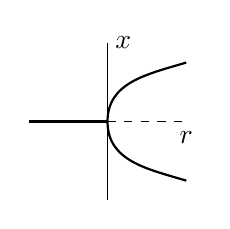
\begin{tikzpicture}
\draw (0,1.5) -- (0,-0.5);
\draw [thick](-1,0.5) -- (0,0.5);
\draw [dashed](0,0.5) -- (1,0.5);
\draw [thick](1,-0.25) .. controls (0.5,-0.1) and (0,0) .. (0,0.5);
\draw [thick](1,1.25) .. controls (0.5,1.1) and (0,1) .. (0,0.5);
\node at (1,0.3) {$r$};
\node at (0.2,1.5) {$x$};
\end{tikzpicture}
\end{center}
\vspace{0.2cm}

\textsc{Subcritical pitchfork bifurcation}\\
Ex: $\dot{x}=rx+x^3$. Only for $r<0$ two unstable fixed points $x^*=\pm \sqrt{-r}$ and stable origin. For $r>0$ origin is unstable (finite escape)
\begin{center}
\begin{tikzpicture}
\draw (0,1.5) -- (0,-0.5);
\draw [thick](-1,0.5) -- (0,0.5);
\draw [dashed](0,0.5) -- (1,0.5);
\draw [dashed](-1,-0.25) .. controls (-0.5,-0.1) and (0,0) .. (0,0.5);
\draw [dashed](-1,1.25) .. controls (-0.5,1.1) and (0,1) .. (0,0.5);
\node at (1,0.3) {$r$};
\node at (0.2,1.5) {$x$};
\end{tikzpicture}
\end{center}

\subsection{Bifurcations of trajectories}













